\documentclass[a4paper,fleqn,12pt]{article}

%%%%%%%%%%%%%%%%%%%%


\usepackage[]{geometry}
\usepackage[latin1]{inputenc}
\usepackage[UKenglish]{babel}
\usepackage[UKenglish]{isodate}
\usepackage{amsmath}
\usepackage{amsfonts}
\usepackage{amssymb}
\usepackage{amsthm}
\usepackage{graphicx}
\usepackage{chngpage}
\usepackage{calc}
\PassOptionsToPackage{hyphens}{url}
\usepackage{hyperref}
\usepackage[nameinlink]{cleveref}
\usepackage{fancyhdr}
\usepackage{titletoc}
\usepackage[explicit]{titlesec}
\usepackage[]{biblatex}
\usepackage[dvipsnames]{xcolor}
\usepackage[sc]{mathpazo}
\linespread{1.05}
\usepackage[T1]{fontenc}
\usepackage{minted}
\usepackage{listings}

\addbibresource{common/bibliography.bib}

\hypersetup{
	colorlinks=true,
	linkcolor=black,
	urlcolor=black,
	citecolor=black
}

\setlength{\parindent}{0mm}
\setlength{\parskip}{\medskipamount}
\renewcommand\baselinestretch{1.2}

\cleanlookdateon

\makeatletter
\newcommand{\@assignment}[0]{Assignment}
\newcommand{\assignment}[1]{\renewcommand{\@assignment}{#1}}
\newcommand{\@supervisor}[0]{}
\newcommand{\supervisor}[1]{\renewcommand{\@supervisor}{#1}}
\newcommand{\@yearofstudy}[0]{}
\newcommand{\yearofstudy}[1]{\renewcommand{\@yearofstudy}{#1}}
\makeatletter

\newtoggle{IsDissertation}

%%%%%%%%%%%%%%%%%%%%%%%%%%%%%%%%%%%%%%%%%%%%%%%%%%%%%%%%%%%%%%%%%%%%%%%%%%%%%%%
%% Project-specific configuration
%%%%%%%%%%%%%%%%%%%%%%%%%%%%%%%%%%%%%%%%%%%%%%%%%%%%%%%%%%%%%%%%%%%%%%%%%%%%%%%

\author{Noah Hollowell}
\title{Visual RISC V Simulator}
% \supervisor{Your supervisor's name}
% \yearofstudy{3\textsuperscript{rd}}

%%%%%%%%%%%%%%%%%%%%%%%%%%%%%%%%%%%%%%%%%%%%%%%%%%%%%%%%%%%%%%%%%%%%%%%%%%%%%%%


\assignment{Project specification}

%%%%%%%%%%%%%%%%%%%%

\pagestyle{plain}
\renewcommand{\headrulewidth}{0.0pt}

\makeatletter
\fancypagestyle{plain}{
	\fancyhf{}
	\fancyhead[R]{\textit{\@title} - \textit{\@assignment}}
    \fancyhead[L]{\textit{\@author}}
    \fancyfoot[C]{\thepage}
}
\makeatother

%%%%%%%%%%%%%%%%%%%%

\begin{document}

\input{../common/titlepage.tex}

\pagestyle{plain}

\section{Introduction/Project Statement}
Within the understanding of how a modern processor works we often look into the underlying code that it runs. However, often being able to visualise
the operations of a processor are far more beneficial to our understanding than simply emulating the physical code.
\\\\
RISC V is a new open source instruction set that has numerous emulators available online with a varying degree of visual elements.
These all lack the ability to fully visualise the internal operations during each instructions execution. Thus, the aim is to produce a fully fledged RISC V simulator that not only emulates RISC V code but also demonstrates exactly what occurs during execution all the way down to bits of data moving across the processor to their respective components that is compliant with the RISC-V specification \cite{risc_spec}

\section{Objectives}
The first part of this project will be to produce a RISC V emulator built in Java. This will require a deep understanding of each RISC V instruction and how each interacts independently within a processor such that they can be combined to produce a logical flow of instructions producing an output.

Objectives include:
\begin{itemize}
    \item A lexical analysis of inputted RISC V code,
    \item A semantic analysis of inputted RISC V code,
    \item Emulation of the base RV32I instruction set as per the RISC V specification,
    \item Emulation of the "Standard Extension for Integer Multiplication and Division" instruction set, \label{obj:md}
    \item Emulation of the "Standard Extension for Single-Precision Floating-Point" instruction set \label{obj:fp}
\end{itemize}

The second part of the project will be to fully visualise the emulator into a simulator providing a fully fledged interface to type and load code, as-well as visualise the internal operation of said code as its runs in real-time.

Objectives include:
\begin{itemize}
    \item A visualisation of the processors register set,
    \item A visualisation of the memory holding both the instructions and data or just data,
    \item A comprehensive system allowing for the display of data moving around the processor including:
    \begin{itemize}
        \item Numerical data moving from memory to other components and vice-versa,
        \item Addressing requests,
        \item Manipulation of multiple values simultaneously to simulate the effect of processor operations (e.g. addition, subtraction, shifts, etc),
    \end{itemize}
    \item Control the speed and steps of the simulation both forwards and backwards in time,
\end{itemize}

To achieve the set out objectives we will approach the project with 2 main overarching goals:
\begin{enumerate}
    \item A minimum viable product that incorporates the base RV64I instruction set and visualisations
    \item A fully fledged product including both the Floating point and Multiplication extensions
\end{enumerate}

And finally an aspirational objective to incorporate more RISC-V extensions dependant of time.


\section{Methods}
In order to successfully develop this project I'll be using a dynamic but structured approach, following along with some of the Agile software methodology and parts of a plan driven approach. This will ensure that all deliverables are produced on time and ensure that a constant flow of progress is achieved with goals in mind and targets to hit.
\\\\
I'll be supplementing development with a series of notes, thus ensuring everything is done and sufficient documentation can be made later in the year.

\subsection{Resources}
The project will be developed entirely in Java 19. This choice was made due to my long running history of development with Java. Java is also highly maintained and constantly updated and has a world-wide community of people providing support at all levels. Java is also architect independent being compiled into byte code that is then run independently on each target device without having to recompile for each target. This is important or this project as the end program needs to be able to run on a range of devices that prospective users may have.
\\\\
To produce the visual front end of the application well be using JavaFX. JavaFX is a more modern GUI library lending itself towards efficient and rapid development which is exactly what I need. Java Swing is also available, however I am more familiar with JavaFX and have already obtained a visual pack called MaterialFX to present a more modern an familiar user interface.
\\\\
To develop the application I'll be making use of Intellij IDEA Ultimate. It's an all in one Java IDE, designed to maximise productivity and prove a wealth of support and debugging tools. I am also familiar with Intellij from previous usage and prefer it over other IDE's such as VSCode for Java due to its highly inter-grated tooling and debugging infrastructure.
\\\\
To ensure thorough testing of the application, I'll be making use of JUnit. JUnit is a testing framework designed for test-driven development and provides a quick and elegant way to produce unit test for all aspects of our application. JUnit is also thoroughly documented and widely used across both the java community and professional development teams.
\\\\
Version control will be done via Git and Github with a additional remote on the DCS systems as an extra backup. I have chosen Git over other Version-Control systems due the the fact that I am more familiar with Git and have extended usage of git.

\subsection{Testing}
Test-driven development (TDD) will be a very important part of the project. As the nature of the project involves emulating individual instructions we can easily apply TDD over all the instructions we aim to implement.
\\\\
Manual testing will also occur for the more visual aspects, in which well ensure that we can visually observe animations taking place at the correct time and in the correct order, also ensuring animated element start and end at the intended place.


\section{Timetable}



\begin{figure}[H]
    \centering
    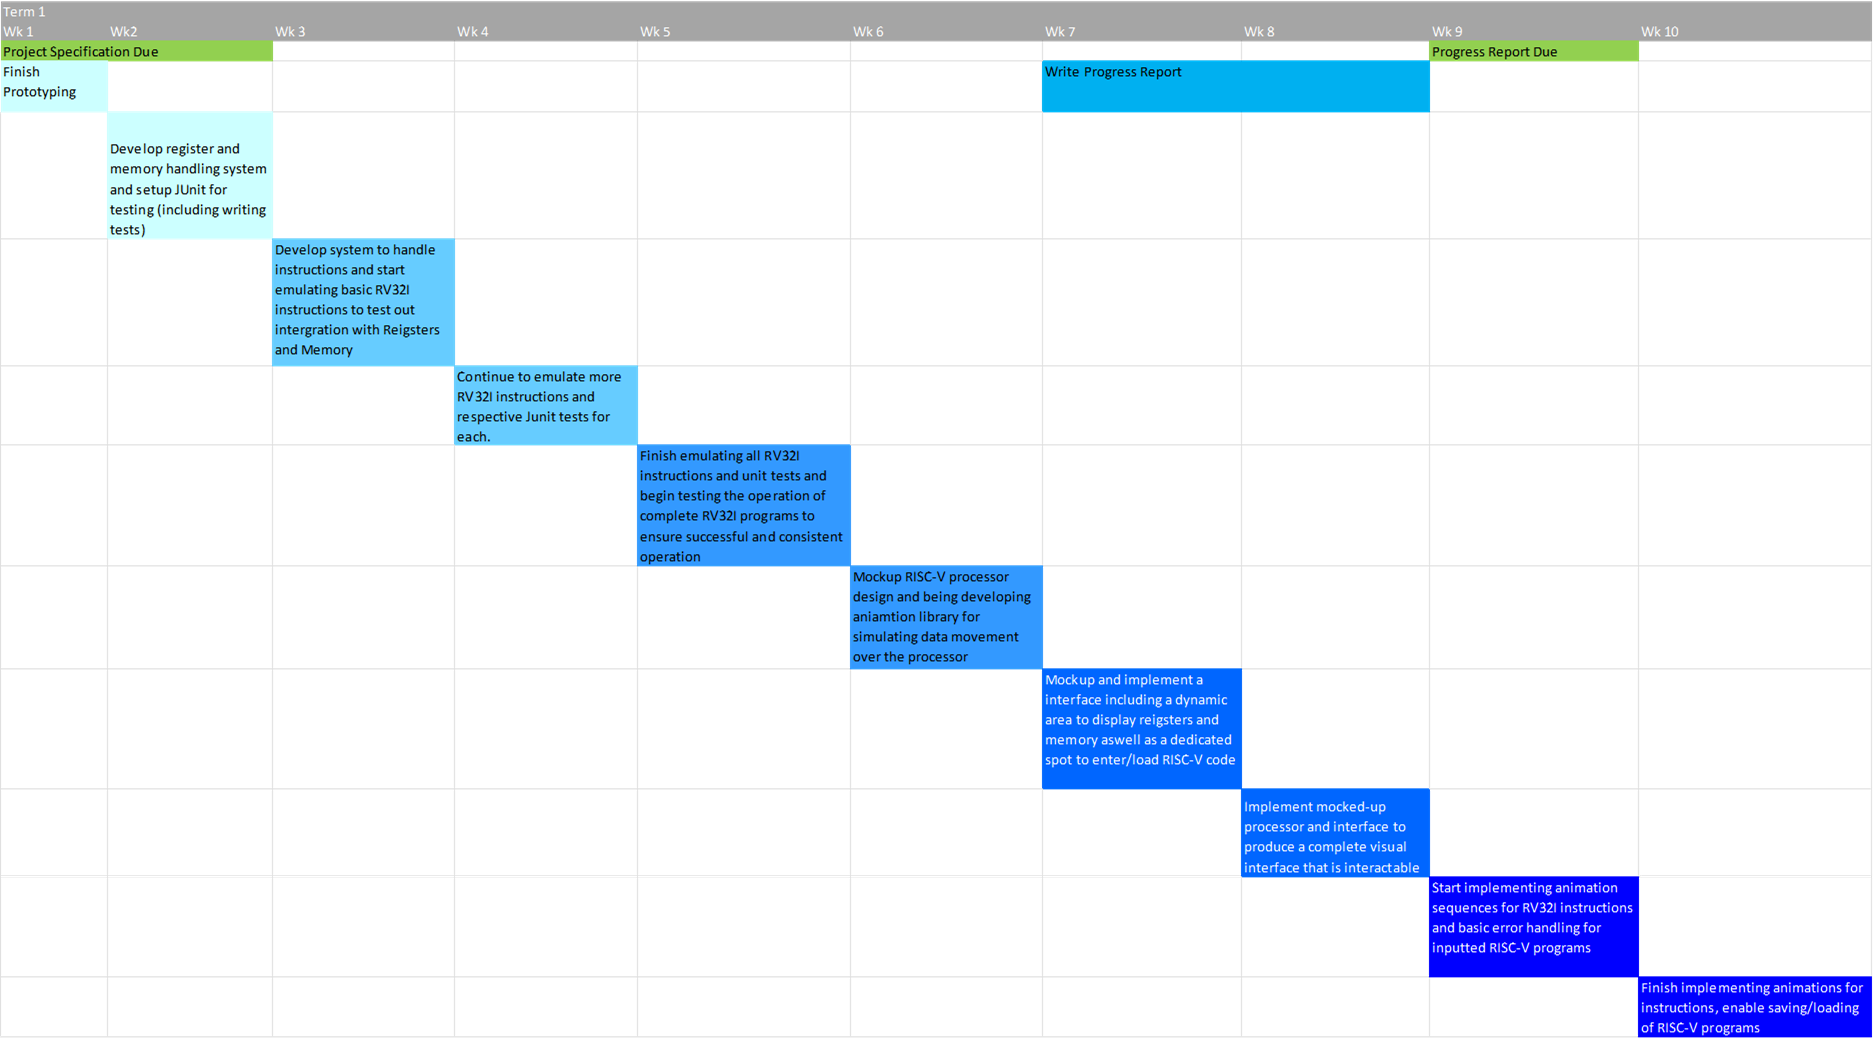
\includegraphics[angle=90, scale=0.68]{specification/t1.png}
    \caption{Term 1 Timetable}
    \label{fig:timetable_t1}
\end{figure}
\begin{figure}[H]
    \centering
    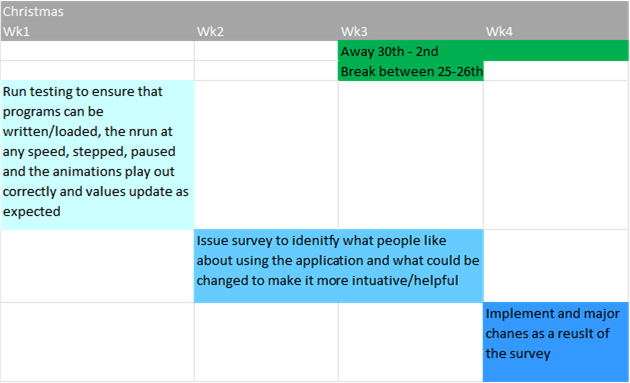
\includegraphics[scale=0.65]{specification/christmas.png}
    \caption{Christmas Timetable}
    \label{fig:timetable_christmas}
\end{figure}
\begin{figure}[H]
    \centering
    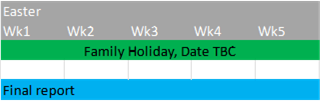
\includegraphics[scale=0.85]{specification/easter.png}
    \caption{Easter Timetable}
    \label{fig:timetable_easter}
\end{figure}
\begin{figure}[H]
    \centering
    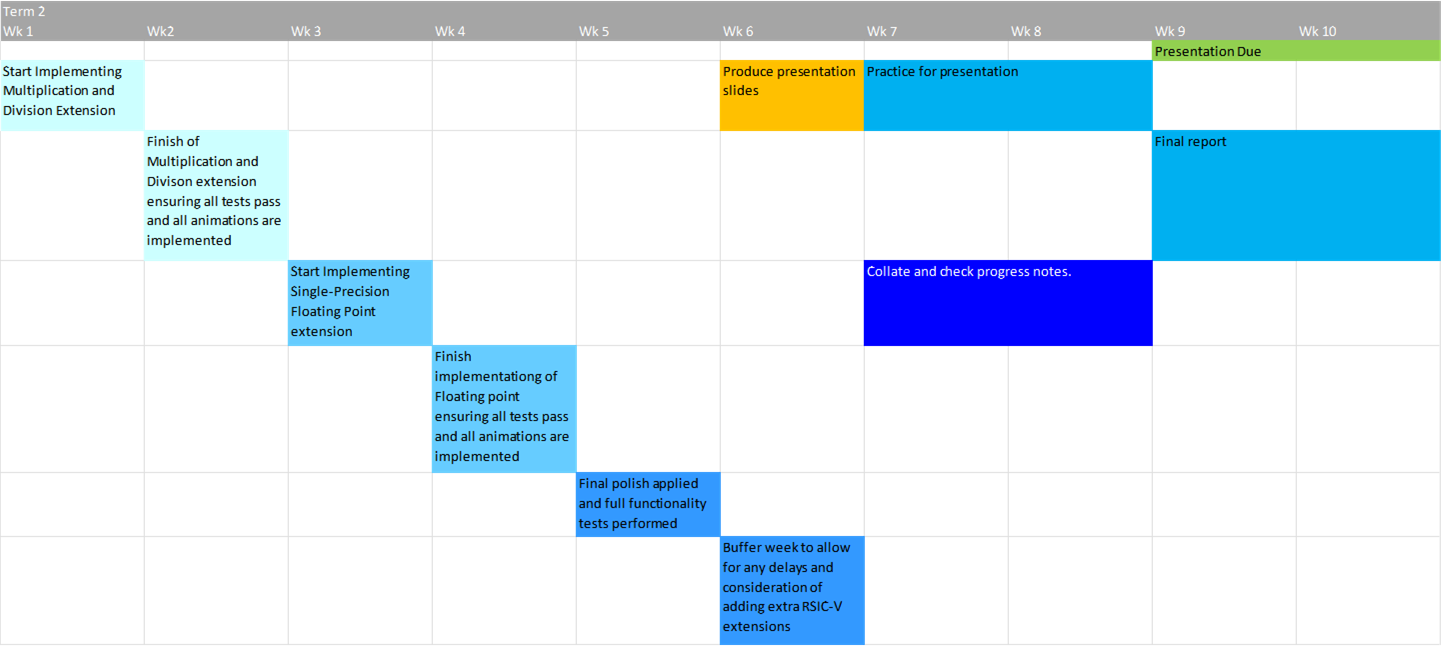
\includegraphics[angle=90, scale=0.75]{specification/t2.png}
    \caption{Term 2 Timetable}
    \label{fig:timetable_t2}
\end{figure}


\section{Risk Assessment}
There is a relatively small amount of risk associated with the project. By having a minimal viable project goal and then a more fully fledged goal we alleviate any risk of ending up with nothing to show and through the spread out nature of implementing sections we can ensure that the entire project will be completed on time with all goals achieved.
\\\\
A possible risk is loosing all code/documentation due to unforeseeable circumstances. However, by making use of Github as a remote and also a remote on DCS, along with zipped backups online I can ensure that there will always be a updated copy of the project available should one become lost, corrupted or unavailable.



\section{Legal, Social, Ethical and Professional Issues}
RISC-V is free and open with a permissive licence. Encourages all implementations are compliant to specification \cite{risc_spec} 
\\\\
Java and its JDK's are available for free use to all users post JDK 16 (we'll be using 19). JavaFX follows the same licence as Java and MaterialFX makes use of the GNU Lesser General Public Licence v3.0 permitting Private and Commercial use.
\\\\
Within surveying for how users find the program we need to consider who we are surveying and why, ensuring no biases are taken to ensure a comprehensive set of feedback from a range of technical backgrounds, and also ensure that the collected information is stored appropriately and disposed of when no longer required.
\\\\
Professionally I'll be sticking to widely known design principles and a professional manner of commenting, ensuring that all comments are related to the code and meaningful.


\bibliographystyle{plain}
\bibliography{common/bibliography}



\end{document}
